\documentclass{standalone}
\usepackage[dvipsnames]{xcolor}
\usepackage{rotating}
\usepackage{tikz}
\usetikzlibrary{positioning, shapes.geometric, shapes.misc, math, calc}

\pgfdeclarelayer{background}
\pgfsetlayers{background,main}

\begin{document}
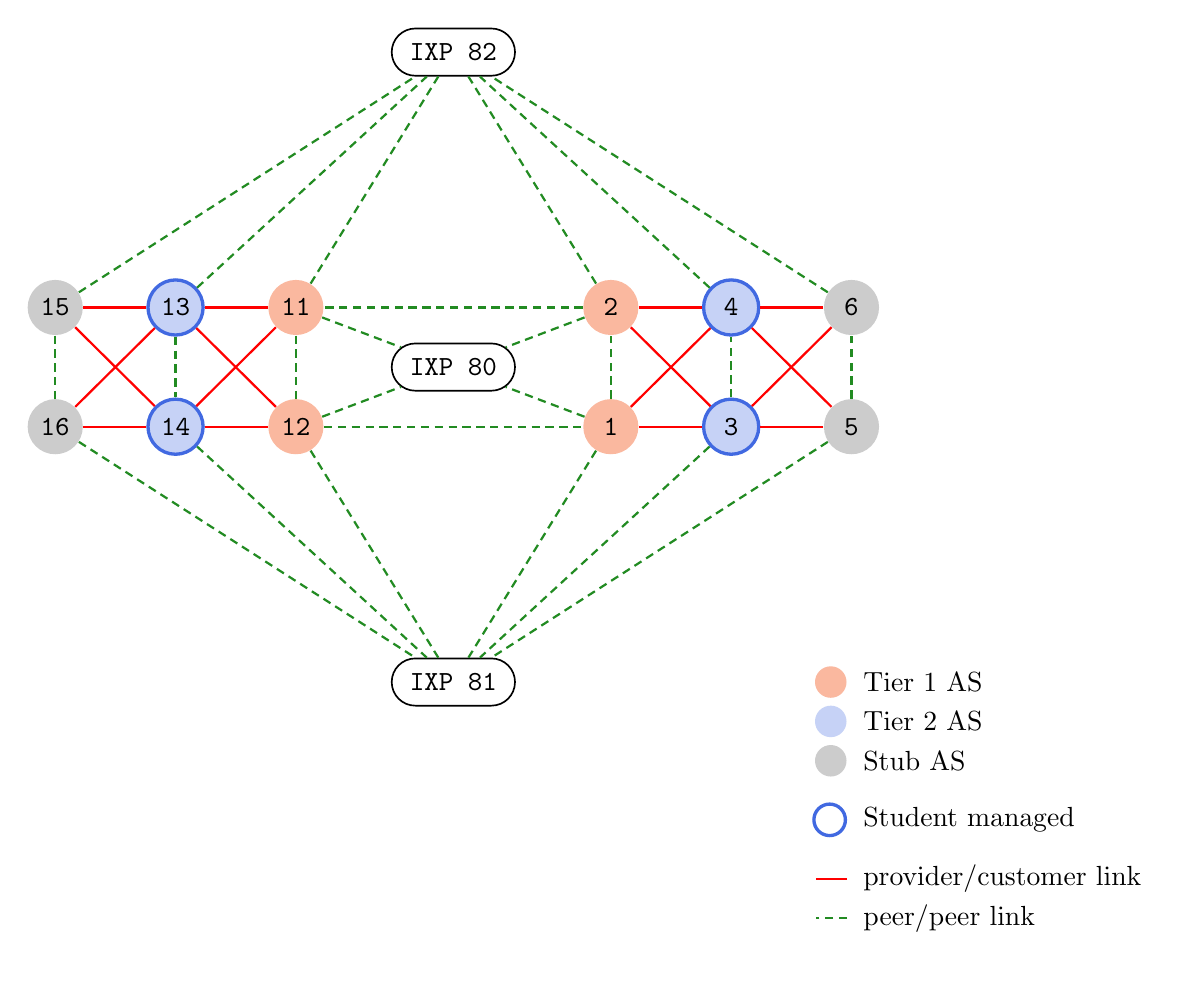
\begin{tikzpicture}[
  % ------------------
  % Styling parameters 
  % ------------------
  % The distance between nodes in a zone.
  node distance=8mm,
  % How to draw all ASes.
  network/.style={draw=none, circle, minimum size=7mm, inner sep=0pt, font={\ttfamily}},
  % Network managed by students
  student managed/.style={draw, very thick, draw=RoyalBlue},
  % Colors for Tier-1 ASes
  tier 1/.style={network, fill=Melon!60},
  % Colors for Tier-2 ASes
  tier 2/.style={network, fill=RoyalBlue!30},
  % Colors for student-managed ASes
  student/.style={tier 2, student managed},
  % Colors for Stub ASes
  stub/.style={network, fill=black!20},
  % Hijack ASes have a different shape,
  hijack/.style={stub, regular polygon, regular polygon sides=6},
  % How to draw IXPs
  ixp/.style={rounded rectangle, draw, fill=white, semithick, minimum height=6mm, minimum width=18mm, font={\ttfamily}},
  % Style of peer2peer links
  peer/.style={draw=ForestGreen, thick, densely dashed},
  % Style of customer-provider links
  prov/.style={draw=Red, thick},
]

% ------------------------------------------------
% Enable Stub Hijacks (adds two ASes to each zone)
% ------------------------------------------------
%\def\EnableStubHijacks{} % Commend this line out to disable.
% -------------------------------
% Make the background transparent
% -------------------------------
\def\TransparentBackground{} % Comment this line out to disable.

\tikzmath{
  integer \zones, \studentAsPerZone, \asPerZone, \zoneStep, \firstIxp, \ixp, \i, \start;
  coordinate \legendPos;
  % -------------
  % Topology size
  % -------------
  \zones = 2;            % Number of zones
  \studentAsPerZone = 2; % Number of configurable ASes per zone.
  \firstIxp = 80;        % The AS number of the first (center) IXP
  \angle = 0;            % Overall angle to rotate the entire picture
  \radiusIxp = 4;        % How far IXPs are from the center IXP.
  \radiusZone = 2;       % How far the tier-1 ASes of each group are from the center IXP.
  \legendPos = (5, -4);  % Location of the legend
}

% -------------------------------------------
% BELOW THIS POINT, NOTHING MUST BE CHANGED.
% -------------------------------------------

\tikzmath{
  \asPerZone = \studentAsPerZone + 4;
  \angleStep = 360 / \zones;
  \zoneStep = 10 * ceil((\asPerZone + 1) / 10);
  \ixp{0} = \firstIxp;
  for \i in {1,..,\zones} {
    \ixp{\i} = \firstIxp + \i;
  };
}
\ifdefined\EnableStubHijacks
  \tikzmath{
    \asPerZone = \asPerZone + 2;
  }
\fi

% Arguments:
% 1. start AS number
% 2. number of ASes in the group
% 3. start coordinate
% 4. rotation
% 5. central IXP
% 6. left IXP
% 7. right IXP
\newcommand{\AREA}[7]{
  \begin{scope}[rotate=#4, transform shape, rot/.style={
      execute at begin node={\begin{turn}{-#4}},
      execute at end node={\end{turn}},
    }]
    \tikzmath{
      integer \s, \t, \start, \last, \step;
      \t1 = #1; \t2 = \t1 + 1;
      \s1 = \t1 + #2 - 2; \s2 = \s1 + 1;
      \start = \t2 + 1;
      \last = \s2;
      \step = \start + 2;
    }
    \node[rot, tier 1, above=4mm of #3] (as\t1) {\t1};
    \node[rot, tier 1, below=4mm of #3] (as\t2) {\t2};
    \draw[peer] (as\t1) -- (#5);
    \draw[peer] (as\t2) -- (#5);
    \draw[peer] (as\t1) -- (#6);
    \draw[peer] (as\t2) -- (#7);
    \draw[peer] (as\t1) -- (as\t2);
    \foreach \n [remember=\n as \p (initially \t1)] in {\start,\step,...,\last}{
      \tikzmath{integer \m, \q; \m = \n + 1; \q = \p + 1;}
      \ifdefined\EnableStubHijacks
        \tikzmath{
          if \n>=\s1 then {
            let \kind = hijack;
          } else {
            if \n>=(\s1-2) then {
              let \kind = tier 2;
            } else {
              let \kind = student;
            };
          };
        }
      \else
        \tikzmath{
          if \n>=\s1 then {
            let \kind = stub;
          } else {
            let \kind = student;
          };
        }
      \fi
      \node[rot, \kind, left=of as\p]  (as\n) {\n};
      \node[rot, \kind, left=of as\q] (as\m) {\m};
      \draw[prov] (as\n) -- (as\p);
      \draw[prov] (as\n) -- (as\q);
      \draw[prov] (as\m) -- (as\p);
      \draw[prov] (as\m) -- (as\q);
      \draw[peer] (as\n) -- (as\m);
      \draw[peer] (as\n) -- (#6);
      \draw[peer] (as\m) -- (#7);
    }
  \end{scope}
}

% Draw all IXPs
\node[ixp] (ixp\ixp{0}) {IXP \ixp{0}};
\foreach [
  evaluate=\i as \theta using (\i-1.5)*\angleStep+\angle
] \i in {1,...,\zones} {
  \node[ixp] at (\theta:\radiusIxp) (ixp\ixp{\i}) {IXP \ixp{\i}};
};

% draw all zones
\foreach [
  evaluate=\i as \theta using (\i-1)*\angleStep+\angle,
  evaluate=\theta as \rotate using 180+\theta,
  evaluate=\i as \start using int(((\i-1)*\zoneStep)+1),
  evaluate=\i as \j using {int(Mod(\i,\zones)+1)},
] \i in {1,...,\zones} {
  \node[coordinate] at (\theta:\radiusZone) (branch\i) {};
  \AREA{\start}{\asPerZone}{branch\i}{\rotate}{ixp\ixp{0}}{ixp\ixp{\i}}{ixp\ixp{\j}}
};

% Ring of tier-1 ASes
\foreach[
  evaluate=\i as \j using {int(Mod(\i,\zones)+1)},
  evaluate=\i as \n using int(((\i-1)*\zoneStep)+2),
  evaluate=\j as \m using int(((\j-1)*\zoneStep)+1),
] \i in {1,...,\zones} {
  \draw[peer] (as\n) -- (as\m);
}

% Legend
\begin{scope}[shift=(\legendPos), yscale=0.5, legend/.style={inner sep=2mm, anchor=west}, small/.style={minimum size=4mm}, local bounding box=legend box]
  \node[legend] at (0,-0) (l1) {Tier 1 AS};  \node[left=0mm of l1, tier 1,  small] {};
  \node[legend] at (0,-1) (l2) {Tier 2 AS};  \node[left=0mm of l2, tier 2,  small] {};
  \node[legend] at (0,-2) (l3) {Stub AS};    \node[left=0mm of l3, stub,    small] {};

  \node[legend] at (0,-3.5) (l4) {Student managed}; \node[left=0mm of l4, student managed, circle,  small] {};
  \ifdefined\EnableStubHijacks
    \node[legend] at (0,-4.5) (l4b) {Malicious AS}; \node[left=0mm of l4b, hijack, thick, small] {};
  \fi

  \ifdefined\EnableStubHijacks \begin{scope}[yshift=-1cm] \fi % shift down everything that follows by 1 unit
  \node[legend] at (0,-5) (l5) {provider/customer link}; \draw[prov] (l5.west) -- ++(-0.4, 0);
  \node[legend] at (0,-6) (l6) {peer/peer link};         \draw[peer] (l6.west) -- ++(-0.4, 0);
  \ifdefined\EnableStubHijacks \end{scope} \fi % close the scope for the shift

  \ifdefined\TransparentBackground
    \begin{pgfonlayer}{background}
      \fill[white] ($(legend box.south west) - (2mm, 2mm)$) rectangle ($(legend box.north east) + (2mm, 2mm)$);
    \end{pgfonlayer}
  \fi
\end{scope}

\begin{scope}[shift={(-7, 3.0)}, transform shape]
\end{scope}


\ifdefined\TransparentBackground
\else
  \begin{pgfonlayer}{background}
    \fill[white] (current bounding box.north west) rectangle (current bounding box.south east);
  \end{pgfonlayer}
\fi

\end{tikzpicture}
\end{document}

%%% Local Variables:
%%% mode: LaTeX
%%% TeX-master: t
%%% End:
